\documentclass{article}
\usepackage{graphicx} % Required for inserting images
\usepackage{amsmath}
\usepackage{amssymb}
\usepackage{float}
\usepackage{textgreek}
\usepackage{fancyhdr}
\usepackage{hyperref}

\usepackage[utf8]{inputenc}
\usepackage{pgfplots}
\usetikzlibrary{intersections, pgfplots.fillbetween}
\pgfplotsset{compat=1.18, width=10cm}

% vnořené popisky obrázků
\usepackage{subcaption}

% automatická konverze EPS 
\usepackage{graphicx} 
\usepackage{epstopdf}

\pagestyle{fancy}



\newcommand\mat[1]{\begin{bmatrix}#1\end{bmatrix}}
\newcommand\pmat[1]{\begin{pmatrix}#1\end{pmatrix}}
\newcommand\vmat[1]{\begin{vmatrix}#1\end{vmatrix}}
\newcommand\pdiff[2]{\frac{\partial #1}{\partial #2}}
\newcommand\hw[1]{\stepcounter{section}\section*{Úkol \thesection\quad #1}}



\title{ARI-HW\_04}
\author{Matěj Pinkas}
\date{16. March 2024}

\lhead{Pinkas Matěj}
\chead{ARI-HW\_04}
\rhead{16. March 2024}


\begin{document}

\maketitle

\section{Příklad}

\begin{itemize}
    \item[-] Pomocí Routh-Hurwitzova kritéria vypočteme stabilitu sytému nasledujícím způsobem
    \begin{align*}
        c(s) &= a_0s^3+a_1s^2+a_2s+a_3\\
        \\
        &\mat{s^3 & a_0 & a_2\\
             s^2 & a_1 & a_3\\
             s^1 & b & c\\
             s^0 & d & e}\\
    \end{align*}
    
    \item[-] systém je stabilní když mají koeficienty $a_0, a_1, b, d$ stejné znaménko
    
    \begin{align*}
        b &= -\frac{\vmat{a_0 & a_2\\ a_1 & a_3}}{a_1} = -\frac{a_0a_3-a_1a_2}{a_1} = \frac{a_1a_2-a_0a_3}{a_1}\\
        c &= -\frac{\vmat{a_0 & 0\\ a_1 & 0}}{a_3} = -\frac{0a_0-0a_1}{a_3}=0\\
        d &= -\frac{\vmat{a_1 & a_3\\ b & c}}{b} = -\frac{a_1c-a_3b}{b} = \frac{a_3b}{b} = a_3\\
        e &= -\frac{\vmat{a_1 & 0\\ b & 0}}{c} = -\frac{0a_1-0b}{c}=0
    \end{align*}
    
    \begin{align*}
        &\mat{s^3 & a_0 & a_2\\
             s^2 & a_1 & a_3\\
             s^1 & \frac{a_1a_2-a_0a_3}{a_1} & 0\\
             s^0 & a_3 & 0}\\
    \end{align*}

    \item[-] Tento postup je aplikován na zadaný systém:

    \begin{align*}
        G(s) &= \frac{1}{(s+1)(s+2)}\\
        K(s) &= \frac{K_ps+K_I}{s}
    \end{align*}
    

    \begin{align*}
        H(s) &= \frac{G(s)K(s)}{1+G(s)K(s)} = 1-\frac{1}{1+G(s)K(s)}=
        1-\frac{1}{1+\frac{K_ps+K_I}{s(s+1)(s+2)}}\\
        &= 1-\frac{1}{\frac{K_ps+K_I+s(s+1)(s+2)}{s(s+1)(s+2)}}=
        1-\frac{s(s+1)(s+2)}{K_ps+K_I+s(s+1)(s+2)}\\
        &= 1-(1-\frac{K_ps+K_I}{K_ps+K_I+s(s+1)(s+2)})=\frac{K_ps+K_I}{K_ps+K_I+s(s+1)(s+2)}
    \end{align*}

    
    \item[-] Z toho charakteristický polynom má tvar:

    \begin{align*}
        K_ps+K_I+s(s+1)(s+2) = s^3+3s^2+(2+K_p)s+K_I
    \end{align*}

    \begin{align*}
        \mat{s^3 & 1 & (2+K_p)\\ 
             s^2 & 3 & K_I\\
             s^1 & \frac{3(2+K_p)-K_I}{3} & 0\\
             s^0 & K_I & 0}
    \end{align*}

    \item[-] $a_0$ je kladá, tedy všechny dašlí hlídané koeficienty musí být kladné aby byl systém stabilní
    
    \begin{align*}
        a_0>0 &\Longleftrightarrow 1>0\\
        a_1>0 &\Longleftrightarrow 3>0\\
        b>0 &\Longleftrightarrow (3(2+K_p)-K_I)/3>0\\
        d>0 &\Longleftrightarrow K_I>0\\
        \\
        K_p>&\frac{K_I}{3}-2
    \end{align*}

    \item[-] Systém je stabilní pro všechny hodnoty $K_I >0$ a zároveň $K_p > \frac{K_I}{3}-2 $ 

    \begin{figure}
        \centering

        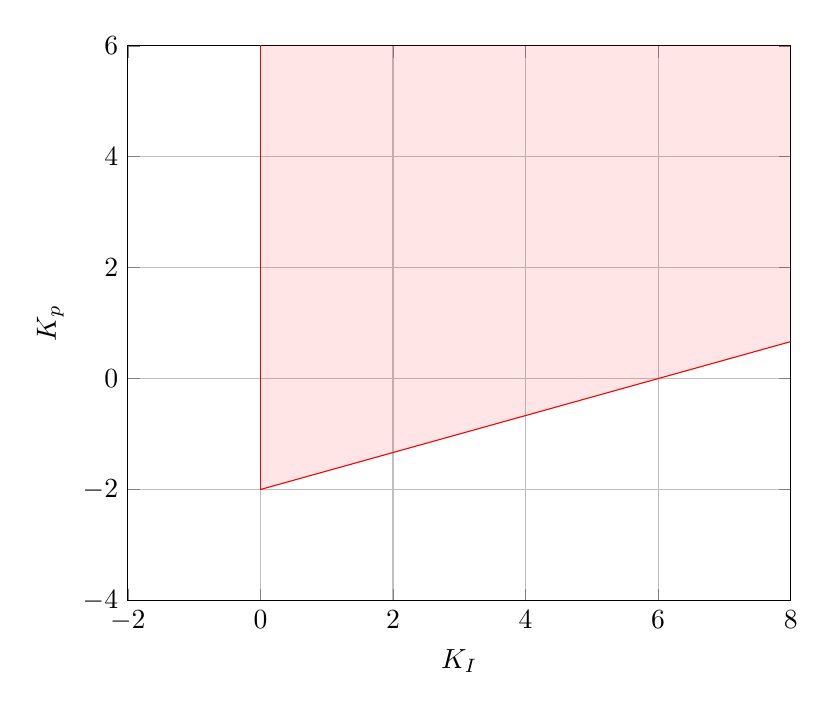
\begin{tikzpicture}
            \begin{axis}[xmin=-2, xmax = 8, ymin = -4, ymax = 6, ylabel=$K_p$, xlabel=$K_I$, grid]
                \addplot[color=red,domain=0:24,name path=linea]{x/3-2};
                \draw[color=red,name path=lineb] (0, -2) -- (0, 10);
                \tikzfillbetween[of=linea and lineb]{red, opacity=0.1};
            \end{axis}
        \end{tikzpicture}
        
        \caption{Oblast koeficientů $K_p$ a $K_I$ pro které je systém stabilní}
        \label{fig:plot 1}
    \end{figure}
\end{itemize}




\newpage
\section{Příklad}

\begin{itemize}
    \item[-] Funkcí hw\_4\_std jsem ze svého datumu narození (10.01.2003) získal systém:
    \begin{align*}
        G(s) = \frac{1}{(s+1)(s+12)}
    \end{align*}
    \item[-] V matlabu pomocí příkazu rltool() vykreslím systém i s vlastním řízením, které pak následně v rltool editoru upravím tak aby póly systému byly co nejdále vlevo od imaginární osy a zároveň dodržely poměrné tlumení $\zeta = 0,7$
    \begin{figure}[H]
        \centering
        \includegraphics[clip, width=1.00\textwidth]{plot.png}
        \caption{rltool graf systému s řízením, vpravo odezva na jednotkový skok}
        \label{fig:plot 2}
    \end{figure}

    \item[-] Z rltool získám po vhodném nastavení nuly a pólů konstantu C

    \begin{align*}
        C(s) &= \frac{45,844(s+1,92)}{s}\\
        K(s) &= \frac{45,844s+88,02048}{s} = 45,844+\frac{88,02048}{s} = K_p + \frac{K_i}{s}\\
        K_p &= 45,844\\ 
        K_i &= 88,02048
    \end{align*}

    \item[-] Systém má (jak je vidět z odezvy na jednotkový skok) nulovou odchylku v době ustálení. Toto můžeme ověřit i tím, že systém je astatický 1. řádu a má tedy nulovou ustálenou odchylku
    
\end{itemize}



\end{document}


